% ==========================================
% step02.tex
% ==========================================
\section{بخش دوم: بهبود کیفیت تصویر به کمک عملگر ضرب ($a \times I$)}

\noindent
عملگر نقطه‌ای $I' = a \times I$ (کشش کنتراست خطی)، بر خلاف عملگر جمع، علاوه بر جابه‌جا کردن میانگین، بر میزان پراکندگی داده‌ها (واریانس و انحراف معیار) نیز تأثیر مستقیم می‌گذارد. ضرب در مقادیر $a > 1$ باعث کشیده شدن هیستوگرام (افزایش کنتراست) و ضرب در مقادیر $a < 1$ باعث فشردگی آن (کاهش کنتراست) می‌شود. در این بخش، تأثیر این عملگر بر روی تصاویر با ضرایب ثابت و سپس با محاسبه ضریب بهینه آماری ارزیابی شده است.

\begin{stepbox}
\field{۱. اعمال ضرایب ثابت $a \in \{0.5, 0.75, 1.25, 1.5\}$ و تحلیل کیفی}{
\textbf{تصویر \texttt{BrightImage} (نیاز به کاهش روشنایی):} ضرب کردن این تصویر در ضرایب بزرگتر از یک ($1.25$ و $1.5$) به دلیل بالا بودن میانگین اولیه، بلافاصله منجر به پدیده \lr{Clipping} در مرز $255$ و از بین رفتن کامل بافت‌ها می‌شود. در مقابل، ضرایب کوچکتر از یک ($0.5$ و $0.75$) هیستوگرام را به سمت مقادیر تاریک‌تر فشرده می‌کنند که باعث بازگشت جزئیات و بهبود کیفیت بصری می‌گردد. 

\textbf{تصویر \texttt{DarkImage} (نیاز به افزایش روشنایی و کنتراست):} از آنجا که هیستوگرام این تصویر در ناحیه تاریک فشرده است، استفاده از ضرایب کوچکتر از یک، آن را تاریک‌تر و غیرقابل‌تشخیص‌تر می‌کند. اما استفاده از ضرایب بسط‌دهنده ($1.25$ و $1.5$)، هیستوگرام را در طول محور روشنایی می‌کشد که نتیجه آن افزایش چشمگیر کنتراست و نمایان شدن بافت‌های پنهان کوهستان است.
}
\end{stepbox}

\begin{figure}[h!]
\centering
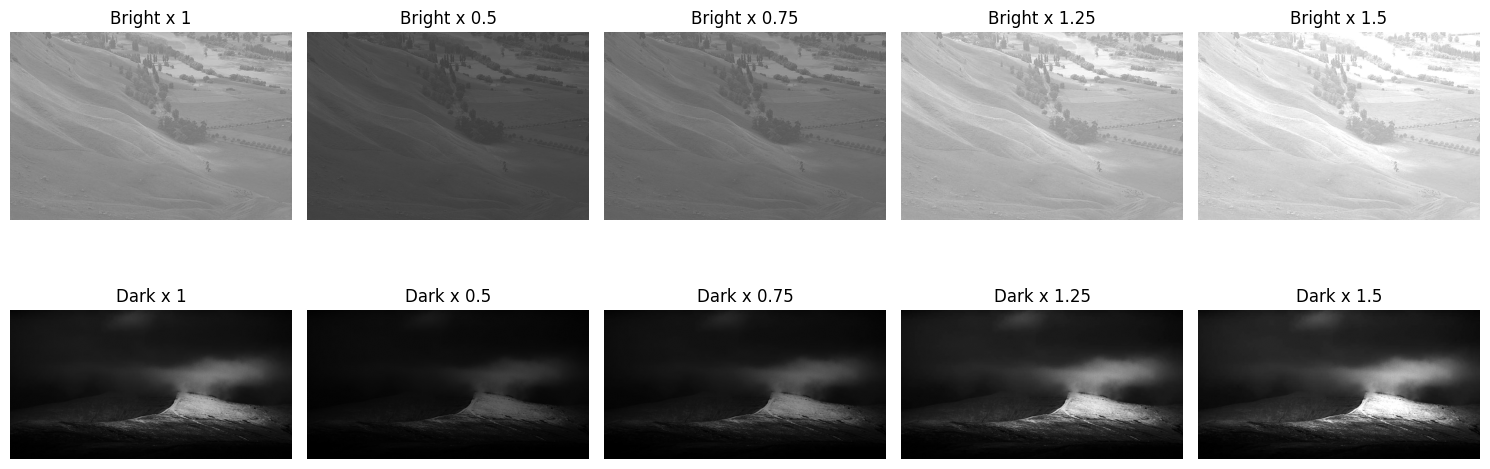
\includegraphics[width=\textwidth]{images/image_2fe39e.png}
\caption{تأثیر اعمال ضرایب ضربی ثابت بر روی هر دو تصویر. ردیف بالا: \texttt{BrightImage}، ردیف پایین: \texttt{DarkImage}}
\label{fig:multipliers_images}
\end{figure}

\begin{figure}[h!]
\centering
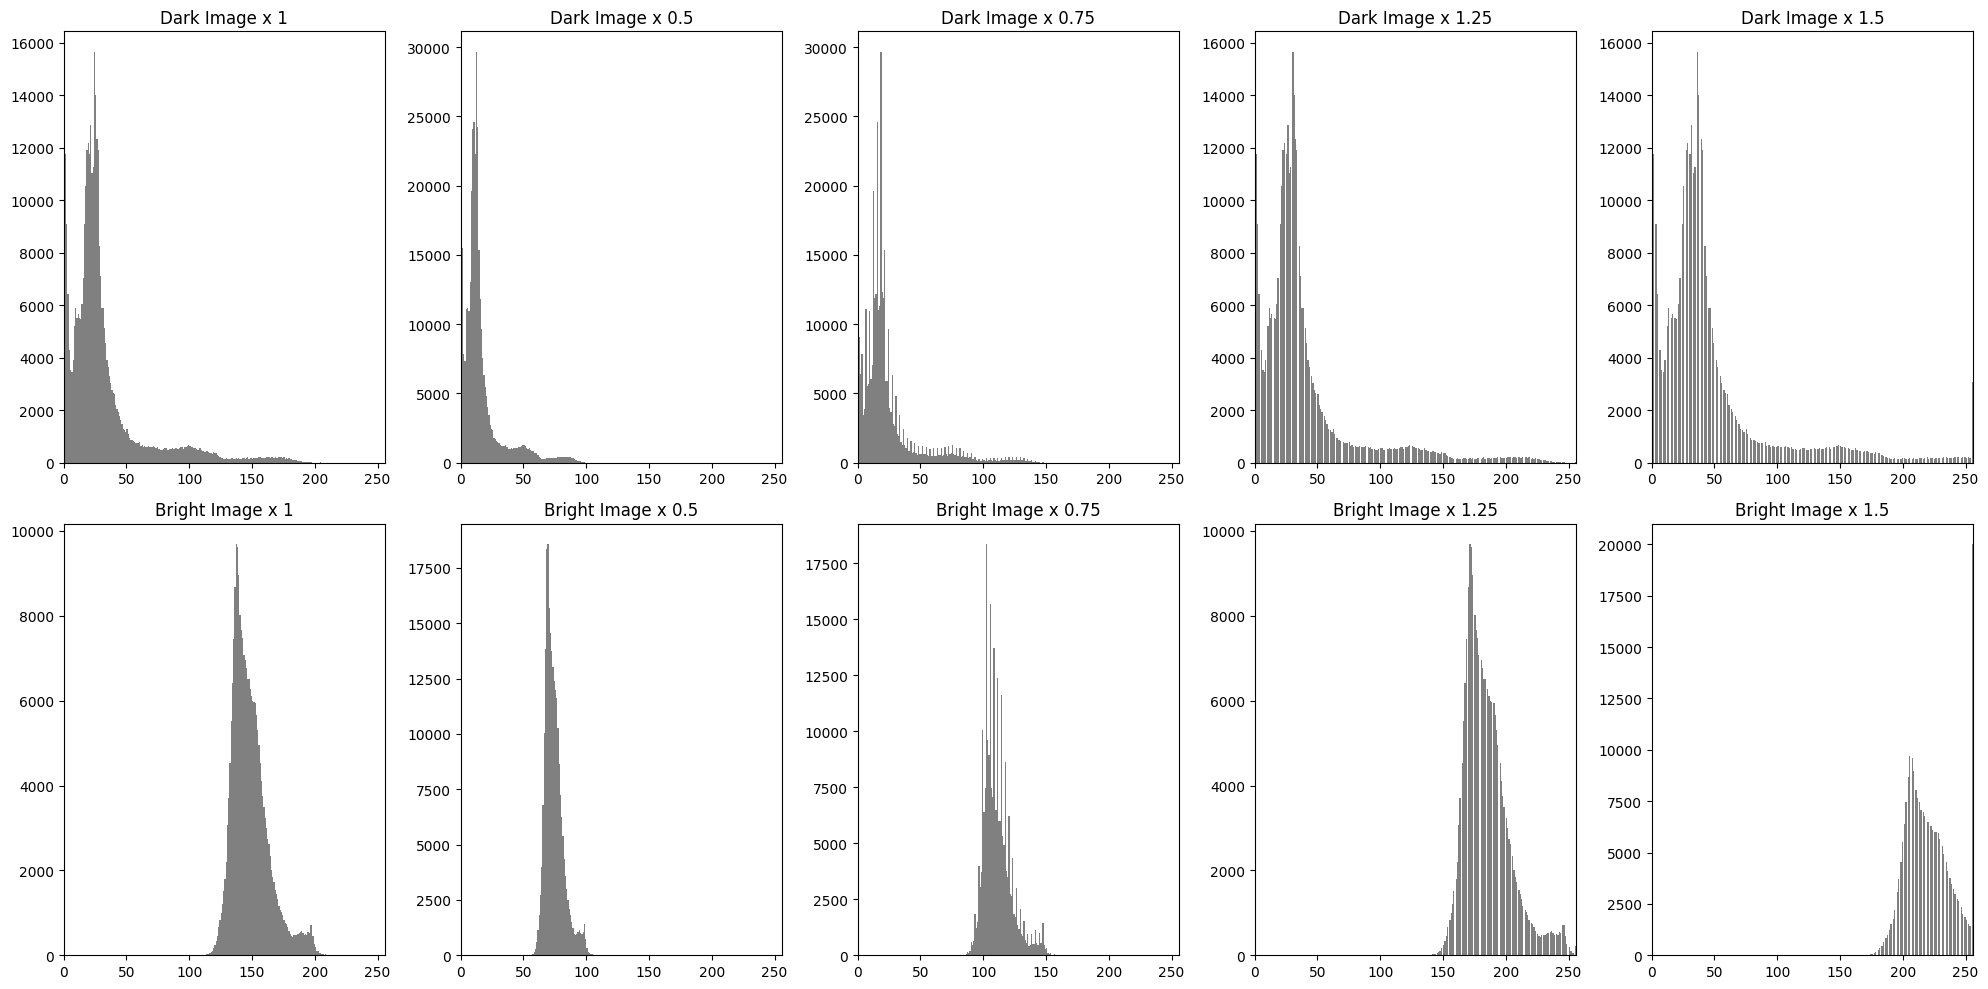
\includegraphics[width=\textwidth]{images/image_2fe3bc.png}
\caption{تغییرات هیستوگرام در اثر عملگر ضرب. همان‌طور که مشخص است، ضرایب $a > 1$ باعث کشیدگی و ضرایب $a < 1$ باعث فشردگی هیستوگرام می‌شوند.}
\label{fig:multipliers_histograms}
\end{figure}

\begin{stepbox}
\field{۲. محاسبه ضریب بهینه ($a_{opt}$) بر اساس انحراف معیار ($\sigma$)}{
انحراف معیار، معیار آماری اصلی برای اندازه‌گیری کنتراست (تضاد نوری) در تصویر است. برای یک تصویر ۸ بیتی ایده‌آل که از تمام ظرفیت دامنه $[0, 255]$ استفاده می‌کند، انحراف معیار هدف را می‌توان بر اساس قانون $4\sigma$ در حدود عدد $64$ (یک‌چهارم بازه) در نظر گرفت. با توجه به رابطه خطی $\sigma_{new} = a \times \sigma_{old}$، ضریب بهینه به صورت زیر محاسبه گردید:
\[
a_{opt} = \left\lceil \frac{64}{\sigma_{current}} \right\rceil
\]
\begin{itemize}[leftmargin=*]
    \item \textbf{برای \texttt{DarkImage}:} با $\sigma \approx 32.34$، ضریب $a_{DI} = 2$ به دست آمد. ضرب کردن تصویر در این عدد، کنتراست آن را دو برابر کرده و هیستوگرام را به خوبی باز کرد.
    \item \textbf{برای \texttt{BrightImage}:} با $\sigma \approx 14.75$، ضریب $a_{BI} = 5$ محاسبه شد. با توجه به اینکه ضرب در ۵ منجر به \lr{Overflow} قطعی می‌شد، از این ضریب به عنوان مقسوم‌علیه ($I / 5$) استفاده گردید تا تصویر به صورت ایمن تاریک شود.
\end{itemize}
}
\end{stepbox}

\begin{codebox}[الگوریتم محاسبه ضریب بهینه آماری]
\begin{lstlisting}[language=Python]
# 64 = 256/4 (Target Standard Deviation)
a_BI = np.ceil(64 / I_BI.std()) # Value: 5.0
a_DI = np.ceil(64 / I_DI.std()) # Value: 2.0

# Apply stretching for dark image and compression for bright image
processed_DI_scaled = np.clip(I_DI * a_DI, 0, 255).astype(np.uint8)
processed_BI_scaled = np.clip(I_BI / a_BI, 0, 255).astype(np.uint8)
\end{lstlisting}
\end{codebox}

\begin{figure}[h!]
\centering
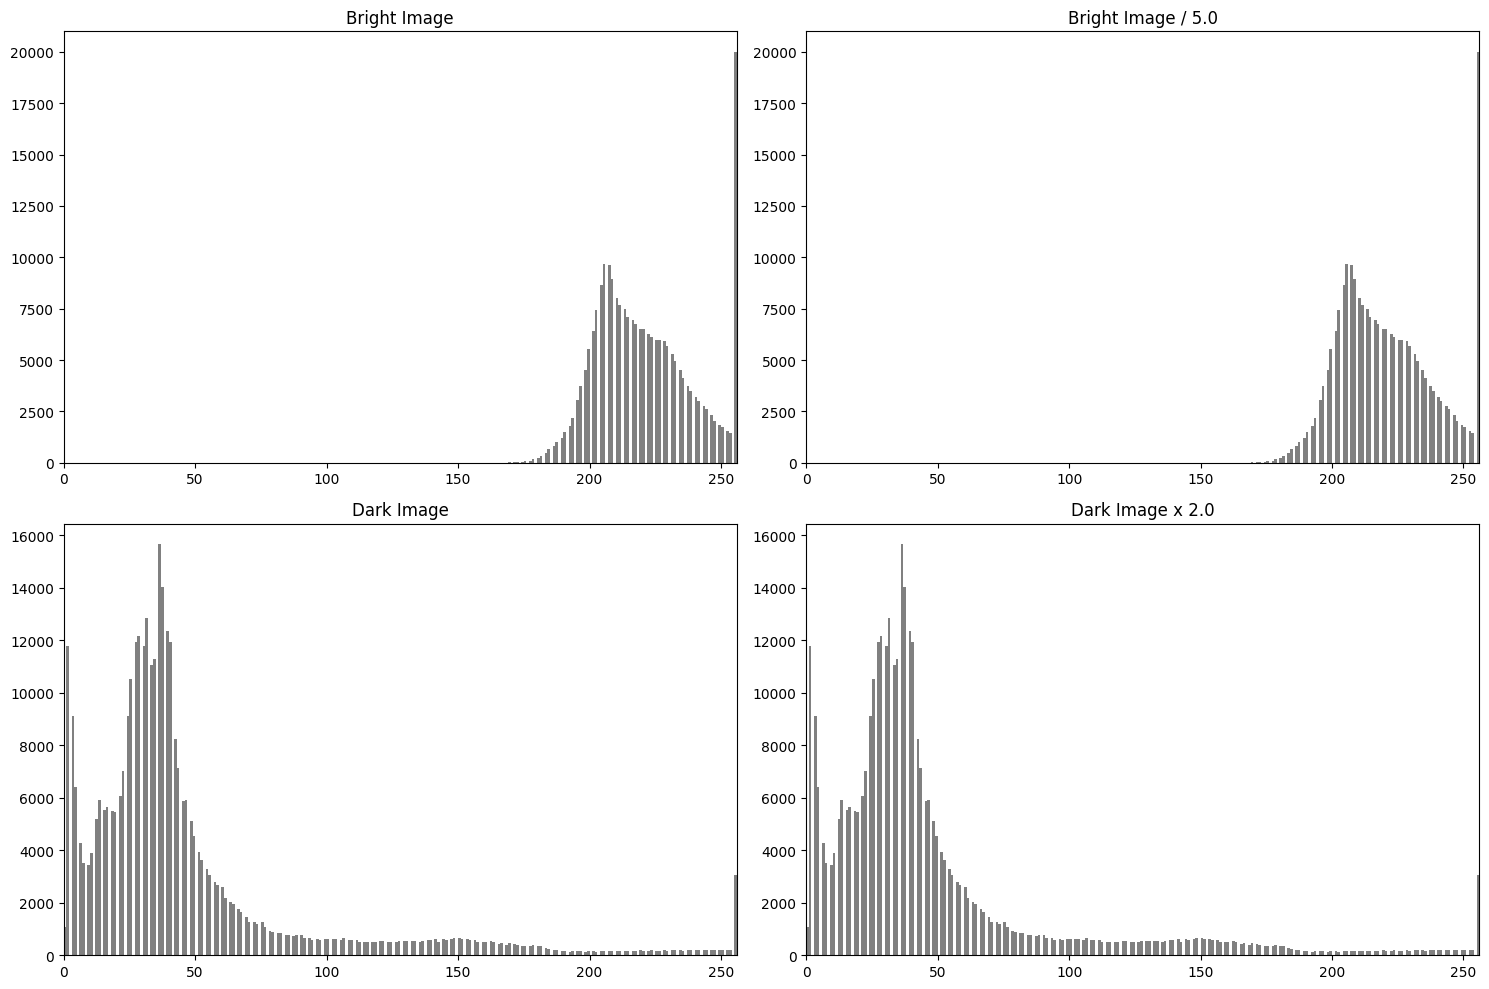
\includegraphics[width=\textwidth]{images/image_2fe382.png}
\caption{نتایج اعمال ضریب بهینه مبتنی بر انحراف معیار. تصویر تاریک در عدد ۲ ضرب شده و تصویر روشن بر عدد ۵ تقسیم شده است.}
\label{fig:optimal_a_images}
\end{figure}

\begin{figure}[h!]
\centering
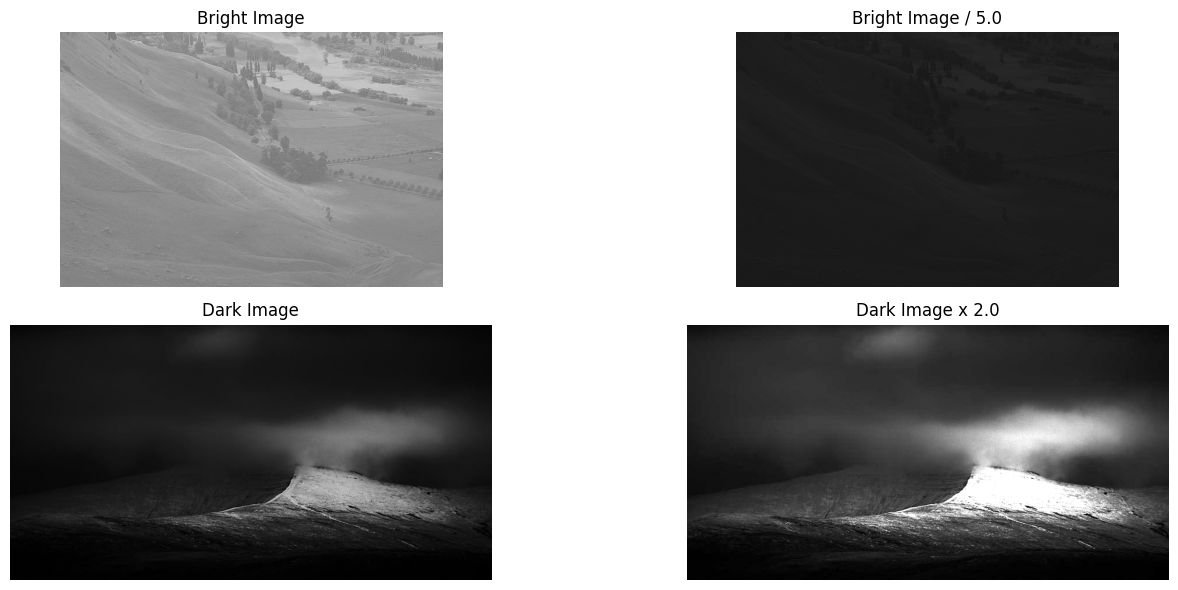
\includegraphics[width=\textwidth]{images/image_2fe3c1.png}
\caption{هیستوگرام تصاویر پس از اعمال ضریب بهینه. در تصویر پایین-راست، کشش کنتراست به وضوح مشهود است.}
\label{fig:optimal_a_histograms}
\end{figure}

\begin{warnbox}[محدودیت ذاتی عملگر ضرب به تنهایی]
استفاده از تقسیم ($I / 5$) برای تصویر روشن، اگرچه مشکل \lr{Clipping} و روشنی مفرط را حل کرد، اما هیستوگرام را به شدت فشرده کرده و کنتراست تصویر را از بین برد (انحراف معیار بسیار پایین آمد). این اتفاق اثبات می‌کند که استفاده از یک عملگر (فقط جمع یا فقط ضرب) به تنهایی برای بهبود کیفیت تصویر کافی نیست. برای داشتن همزمان روشنایی متعادل و کنتراست بالا، به انتقال افاین (Affine) یعنی فرمول $a \times I + b$ نیاز داریم.
\end{warnbox}